% $Header: /Users/joseph/Documents/LaTeX/beamer/solutions/conference-talks/conference-ornate-20min.en.tex,v 90e850259b8b 2007/01/28 20:48:30 tantau $

\documentclass{beamer}

\usefonttheme{professionalfonts}%  don't change fonts inside beamer
% This file is a solution template for:

% - Talk at a conference/colloquium.
% - Talk length is about 20min.
% - Style is ornate.



% Copyright 2004 by Till Tantau <tantau@users.sourceforge.net>.
%
% In principle, this file can be redistributed and/or modified under
% the terms of the GNU Public License, version 2.
%
% However, this file is supposed to be a template to be modified
% for your own needs. For this reason, if you use this file as a
% template and not specifically distribute it as part of a another
% package/program, I grant the extra permission to freely copy and
% modify this file as you see fit and even to delete this copyright
% notice. 


\mode<presentation>
{
  % \usetheme{Warsaw}
  % or ...

  \setbeamercovered{transparent}
  % or whatever (possibly just delete it)
}


%\usepackage[english]{babel}
% or whatever

%\usepackage[latin1]{inputenc}
% or whatever
\usepackage{polyglossia}
\setmainlanguage{english}
\usepackage{fontspec}
\usepackage{xeCJK}
\usepackage{unicode-math}
	\setmathfont{Latin Modern Math} % default
	%\setmathfont[range=\mathalpha]{Asana Math}
	\setmathfont{Asana Math}[range={\mathbin}] %\mathord
	\setmathfont{STIX Math}[range={"02609}] % ☉
	\setmathfont{XITS Math}[range={"1D4B6-"1D4CF}] % Script, Latin, lowercase
	\setmathfont{Latin Modern Math}[range={"1D608-"1D63B}, sans-style=italic]
	\setmathfont{Latin Modern Math}[range={
		"00391-"003A9,
		"003B1-"003F5, 
		"1D6A8-"1D6E1},	% Bold Greek
		sans-style=upright]
		
	%\setmathfont{⟨font name⟩}[range=⟨unicode range⟩,⟨font features⟩]
\usepackage{siunitx}
% ':=' as \coloneqq
%\usepackage{mathtools}
\usepackage{empheq} % numcases


%\usepackage{times}
%\usepackage[T1]{fontenc}
% Or whatever. Note that the encoding and the font should match. If T1
% does not look nice, try deleting the line with the fontenc.


\title%[Short Paper Title] % (optional, use only with long paper titles)
{An Introduction to \cite{Wang2017}}

\subtitle{An Attempt to Avoid the Old Cosmological Constant Problem}

\author[Wang] % (optional, use only with lots of authors)
{Yi-Fan Wang (王\ 一帆)}
%\inst{1} \and %S.~Another\inst{2}}
% - Give the names in the same order as the appear in the paper.
% - Use the \inst{?} command only if the authors have different
%   affiliation.

\institute[Uni zu Köln] % (optional, but mostly needed)
{
  %\inst{1}%
	Institut für Theoretische Physik\\
	Universität zu Köln}
  %\and
  %\inst{2}%
  %Department of Theoretical Philosophy\\
  %University of Elsewhere}
% - Use the \inst command only if there are several affiliations.
% - Keep it simple, no one is interested in your street address.

\date%[BCGS Admission 2017]
% (optional, should be abbreviation of conference name)
{June 20, 2017}
% - Either use conference name or its abbreviation.
% - Not really informative to the audience, more for people (including
%   yourself) who are reading the slides online

\subject{General Relativity and Cosmology}
% This is only inserted into the PDF information catalog. Can be left
% out. 



% If you have a file called "university-logo-filename.xxx", where xxx
% is a graphic format that can be processed by latex or pdflatex,
% resp., then you can add a logo as follows:

\pgfdeclareimage[height=1.0cm]{university-logo}%
{./logos/uni-koeln/UzK_Logo_ger.pdf}
\logo{\pgfuseimage{university-logo}}



% Delete this, if you do not want the table of contents to pop up at
% the beginning of each subsection:
\AtBeginSection[]
{
  \begin{frame}<beamer>{Outline}
    \tableofcontents[currentsection,currentsubsection]
  \end{frame}
}


% If you wish to uncover everything in a step-wise fashion, uncomment
% the following command: 

%\beamerdefaultoverlayspecification{<+->}

\usepackage[citestyle=alphabetic,doi=false,isbn=false,url=false,
defernumbers=true]%
	{biblatex}
\addbibresource{cosmo-const.bib}

\usepackage{tikz}
% \usepackage{tikz-3dplot}
% \usetikzlibrary{positioning,shapes,arrows}
\usetikzlibrary{decorations.pathmorphing}
\usetikzlibrary{calc}
% \usetikzlibrary{decorations.markings}

\usepackage{pgfplots}
\pgfplotsset{compat=1.13}
\usepgfplotslibrary{fillbetween}

\usepackage{cleveref}

\usepackage{braket}

\input{./preambles/math-single}
\input{./preambles/math-brac}
\input{./preambles/phys-chem}

\begin{document}

\begin{frame}
  \titlepage
\end{frame}

\begin{frame}{Outline}
  \tableofcontents
  % You might wish to add the option [pausesections]
\end{frame}


% Structuring a talk is a difficult task and the following structure
% may not be suitable. Here are some rules that apply for this
% solution: 

% - Exactly two or three sections (other than the summary).
% - At *most* three subsections per section.
% - Talk about 30s to 2min per frame. So there should be between about
%   15 and 30 frames, all told.

% - A conference audience is likely to know very little of what you
%   are going to talk about. So *simplify*!
% - In a 20min talk, getting the main ideas across is hard
%   enough. Leave out details, even if it means being less precise than
%   you think necessary.
% - If you omit details that are vital to the proof/implementation,
%   just say so once. Everybody will be happy with that.

\section{Overview}

\begin{frame}{Overview}
\begin{itemize}
\item If contributed by vacuum energy, the cosmological constant could
\alert{differ \num{120} order-of-magnitude} from observation.
\item \citeauthor{Wang2017} consider vacuum energy \alert{density} instead, 
which is subject to \alert{fluctuation}, and their results could moderate the 
problem.
\item They assumed a \alert{localised RW metric} and obtained FL-like equations 
for $\rfun{a}{t,\vec{x}}$, whose coefficient contains fluctuation, which is 
evaluated from QFT in flat space-time.
\item The equations leads to local Hubble parameters which fluctuate, but a
global average is claimed be defined.
\item The solution to the equations is evaluated with various approximations.
\item The results are qualitatively supported by numerical calculation and 
further discussion.
\end{itemize}

\end{frame}


\section{The Old Cosmological Constant Problem}

\begin{frame}{Cosmological constant and vacuum energy}
\begin{itemize}
\item GR + vacuum QFT
\begin{equation}
G_{\mu\nu} + \lambda_\text{b} g_{\mu\nu} = 8\pp\nG T^\text{vac}_{\mu\nu}
\label{eq:1}
\end{equation}
\item In Special Relativity, Lorentz invariance requires
\begin{equation}
T^\text{vac}_{\mu\nu} = -\rho^\text{vac}_{\mu\nu} \eta_{\mu\nu},
\end{equation}
which generalises to curved space-time as
\begin{equation}
T^\text{vac}_{\mu\nu} = -\rho^\text{vac}_{\mu\nu} g_{\mu\nu}.
\end{equation}
\item Effectively, \cref{eq:1} can be written as
\begin{align}
G_{\mu\nu} + \lambda_\text{eff} g_{\mu\nu} = 0, \qquad
\lambda_\text{eff} \coloneqq \lambda_\text{b} + 8\pp\nG\rho^\text{vac};
\label{eq:Einstein-2}\\
G_{\mu\nu} = -8\pp\nG\rho^\text{vac}_\text{eff} g_{\mu\nu}, \qquad
\rho^\text{vac}_\text{eff} \coloneqq \rho^\text{vac} +
\frac{\lambda_\text{b}}{8\pp\nG}.
\label{eq:Einstein-3}
\end{align}
\end{itemize}
\end{frame}

\begin{frame}{Hubble parameter and cosmological constant}
\begin{itemize}
\item Homogeneity and isotropy: Robertson--Walker metric
\begin{equation}
\dd s^2 = -\dd t^2 + \rfun{a^2}{t}\,\delta_{ij}\,\dd x^i\,\dd x^j.
\end{equation}
\item Hubble parameter / expansion rate $\hH \coloneqq \dot{a}/a$;
\cref{eq:Einstein-2,eq:Einstein-3} take the corresponding Friedmann--Lemaître
form
\begin{align}
3\hH^2 = \lambda_\text{eff} = 8\pp\nG\rho^\text{vac}_\text{eff},\\
3\ddot{a} = \lambda_\text{eff} a = 8\pp\nG\rho^\text{vac}_\text{eff} a.
\label{eq:FL-2}
\end{align}

\item Solution to \cref{eq:FL-2}
\begin{equation}
\rfun{a}{t} = \rfun{a}{t_0}\,\ee^{\hH \rbr{t-t_0}}
\end{equation}

\end{itemize}

\end{frame}

\begin{frame}{The Old Cosmological Problem}
\begin{itemize}

\item Contributions to $\rho^\text{vac}_\text{eff}$ or $\lambda_\text{eff}$:
vacuum fluctuation of all quantum fields, Electroweak phase transition, etc.

\item $\lambda_\text{eff}$ by vacuum fluctuation evaluated in Minkowski space:
taking a \alert{scalar field} (also see below) and using sharp-momentum cut-off,
\begin{equation}
\left<\rho^\text{vac}\right> = \frac{\varLambda^4}{16\pp^2}.
\end{equation}
\item Setting $\varLambda = E_\text{P}$ results in a surpass of the observed 
value of $\lambda_\text{eff}$ by a factor of $\sim 10^{120}$.

\end{itemize}

\end{frame}

\section{Matter and space-time models}

\begin{frame}{Matter: field and quantisation}

\begin{itemize}
\item Matter model: free neutral massless scalar field in flat space-time
\begin{equation}
\sfun{S_\text{m}}{\phi} \coloneqq \int \dd^4 x\,\sbr{-\frac{1}{2}\eta^{\mu\nu}
\rbr{\partial_\mu \phi}\rbr{\partial_\nu \phi}}
\label{eq:matter-classical}
\end{equation}
\item Canonical quantisation
\begin{equation}
\rfun{\phi}{t,\vec{x}} \coloneqq \int\frac{\dd^3 k}{\rbr{2\pp}^{3/2}} 
\frac{1}{\sqrt{2\omega}}
\rbr{a_{\vec{k}} \,\ee^{-\ii\rbr{\omega t - \vec{k}\cdot\vec{x}}} + 
\text{h.c.}},
\label{eq:matter-quantised}
\end{equation}
so that
\begin{align}
T_{00} &= \frac{1}{2}\rbr{\dot{\phi}^2 + \rbr{\nabla\phi}^2} \\
&= \int\dd^3 k_1\,\dd^3 k_2\,
\rfun{f}{a_{\vec{k}_1} a_{\vec{k}_2}^\dagger, a_{\vec{k}_1}^\dagger 
a_{\vec{k}_2}, \alert{a_{\vec{k}_1} a_{\vec{k}_2}, a_{\vec{k}_1}^\dagger 
a_{\vec{k}_2}^\dagger}}
\end{align}
\end{itemize}


\end{frame}

\begin{frame}{Matter: fluctuating vacuum energy density}
\begin{itemize}
\item Hamiltonian
\begin{equation}
H \coloneqq \int \dd^3 x\,T_{00} = \frac{1}{2}\int \dd^3 k\,\omega\rbr{a_{\vec 
k}a_{\vec k}^\dagger + a_{\vec k}^\dagger a_{\vec k}}.
\end{equation}

\item $\Ket{0}$ is an eigenstate of $H$, because it is defined by
\begin{equation}
a_{\vec k} \Ket{0} \coloneqq 0,\quad \forall \vec k
\end{equation}
\item This is not the case for $T_{00}$, and one has
\begin{equation}
\abr{\rbr{\Delta T_{00}}^2} = \frac{2}{3}\abr{T_{00}}^2,\qquad \abr{T_{00}} = 
\frac{\varLambda^4}{16\pp^2}.
\end{equation}

\end{itemize}

\end{frame}


\begin{frame}{Space-time: localised Robertson--Walker metric}
\begin{itemize}
\item \alert{In}homogeneity and isotropy
\begin{empheq}[box=\fbox]{equation}
\dd s^2 \coloneqq -\dd t^2 + \rfun{a}{t, \alert{\vec{x}}}
\,\delta_{ij}\,\dd x^i\,\dd x^j.
\end{empheq}
\item Generalising the proper distance and Hubble parameter
\begin{equation}
\rfun{L_{1\to 2}}{t} \coloneqq \int_{\vec x_1}^{\vec 
x_2}\sqrt{\rfun{a^2}{t,\vec x}}\,\dd l,\quad
\rfun{\hH_{1\to 2}}{t} \coloneqq \frac{\dot L_{1\to 2}}{L_{1\to 2}}
\end{equation}

\item Einstein equations
\begin{equation}
G_{\mu\nu} = 8\pp\nG T_{\mu\nu},
\label{eq:E-20}
\end{equation}
where $T_{\mu\nu}$'s are viewed as (random c-)numbers (and subject to 
fluctuation)
\end{itemize}


\end{frame}

%\begin{frame}{Space-time: fluctuating scale-factor}
%\begin{itemize}
%\item $\rbr{0i}$-component of Einstein equations
%\begin{equation}
%\partial_i \frac{\dot{a}}{a} = -4\pp\nG T_{0i},
%\end{equation}
%the solution to which reads
%\begin{equation}
%\fat{\frac{\dot{a}}{a}}{\vec x} = \fat{\frac{\dot{a}}{a}}{\vec x_0}
%- 4\pp\nG \int_{\vec x_0}^{\vec x}T_{0i}\,\dd x^i
%\end{equation}
%\item

%\end{itemize}


%\end{frame}

\begin{frame}{Space-time: stochastic oscillator equation for $a$}
\begin{itemize}
\item Taking the trace of \cref{eq:E-20} leads to
\begin{empheq}[box=\fbox]{equation}
\ddot a + \rfun{\Omega^2}{t,\vec x}\, a = 0,
\label{eq:sho}
\end{empheq}
where
\begin{equation}
\Omega^2 \coloneqq \frac{4\pp\nG}{3} g^{\mu\nu} T_{\mu\nu},
\end{equation}
which is viewed as a (random c-)number (and subject to fluctuation)

\item $T_{\mu\nu}$ given by the quantised scalar field 
\cref{eq:matter-classical,eq:matter-quantised}; evaluate Hubble parameter by 
solving \cref{eq:sho}
\end{itemize}

%\begin{itemize}
%\item Connecting different spacial points: read the paper
%\end{itemize}

\end{frame}

\section{Solving $\rfun{a}{t,\vec{x}}$: parametric oscillator}

\begin{frame}{Parametric oscillator}
\begin{itemize}
\item If $\Omega$ were definite and periodic in $t$, \cref{eq:sho} would be 
a Hill's equation, describing \alert{parametric oscillation} (see e.g.\ 
\cite[§27]{Landau1976} and Wikipedia)
\item General solution
\begin{equation}
\rfun{a}{t,\vec x} = c_1 \ee^{\alert{+}\hH_{\vec x}t}\rfun{P_1}{t,\vec x}
+ c_2 \ee^{\alert{-}\hH_{\vec x}t}\rfun{P_2}{t,\vec x}
\end{equation}
where $\hH_{\vec x} > 0$ (thus second term exponentially suppressed at late 
time) and $P_i$'s have the same period as $\Omega$.
\item It was claimed that $\Omega$ behaves \alert{quasi-periodically}, because 
of $\sfun{\mathrm{Cov}}{\rfun{\Omega^2}{t_1, \vec x}, 
\rfun{\Omega^2}{t_2, \vec x}}$ (see below)

\end{itemize}


\end{frame}

\begin{frame}{Quasi-periodicity}
\begin{itemize}
\item Covariance of $\rfun{\Omega^2}{t}$, taken from \cite{Wang2017}
\begin{center}
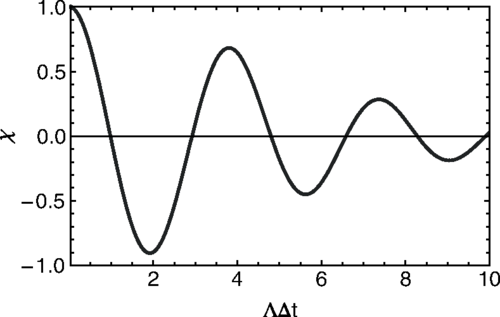
\includegraphics[width=.6\linewidth]{./graphics/FIG.2.png}
\end{center}
\item The solution is modified (at late time) to be
\begin{empheq}[box=\fbox]{equation}
\rfun{a}{t,\vec x} \approx \ee^{\alert{\int_0^t \dd}t'\, \rfun{\hH_{\vec 
x}}{t'}}
\rfun{P}{t,\vec x},
\label{eq:approx-a}
\end{empheq}
where $\rfun{P}{t,\vec x}$ behaves also only \alert{quasi-}periodically (see 
below).

\end{itemize}

\end{frame}

\begin{frame}{Proper distance and Hubble parameter revisited}
\begin{itemize}
\item The expressions for proper distance and Hubble parameter in terms of 
\cref{eq:approx-a} are
\begin{equation}
\rfun{L_{1\to 2}}{t} = \rfun{L_{1\to 2}}{0}\,\ee^{\hH t},\quad
\rfun{L_{1\to 2}}{0} =
\int_{\vec x_1}^{\vec x_2} \sqrt{\rfun{P^2}{t,\vec x}}\,\dd t,
\end{equation}
\begin{empheq}[box=\fbox]{equation}
\hH = \frac{1}{t} \int_0^t \rfun{\hH_{\vec x}}{t'}\,\dd t'.
\end{empheq}
\item It looks like that the authors assumed averaging over a long distance 
/ time smooths out the difference between different $\vec x$.

\item It was claimed that leading-order WKB gives
\begin{equation}
\rfun{a}{t,\vec x} \approx \frac{A_0}{\sqrt{\Omega}}
\rfun{\cos}{\alert{\int_0^t\dd}t'\,\rfun{\Omega}{t', \vec x}+ 
\theta_{\vec x}}.
\label{eq:wkb-sol}
\end{equation}

\end{itemize}

\end{frame}



\section{Solving $\rfun{a}{t,\vec{x}}$: adiabatic approximation}

\begin{frame}{Review: canonical transformation}
\begin{itemize}
\item Introducing the (type-2) generating function $\rfun{G_2}{q, P, t}$
\begin{equation}
S = \int p\,\dd q - H \,\dd t
\equiv \int P\,\dd Q - K\,\dd t + \dd \rbr{-QP + G_2}
\end{equation}
where $H = \rfun{H}{q, p, t}$, $K = \rfun{K}{Q, P, t}$, so that
\begin{equation}
\int \rbr{p - \partial_q G_2}\,\dd q + \rbr{Q - \partial_P G_2}\,\dd P 
+ \rbr{K - H + \partial_t G_2}\,\dd t\equiv 0.
\end{equation}
\item Arbitrariness of the track in phase space requires
\begin{equation}
p = \partial_q G_2,\quad
Q = \partial_P G_2,\quad
K = H - \partial_t G_2.
\end{equation}
\item It can be shown that $G_2$ generates a Possion-bracket-keeping 
transformation from $\rbr{q, p; H}$ to $\rbr{Q, P; K}$.
\end{itemize}
\end{frame}

\begin{frame}{Action-angle variables}{See e.g.\ \cite{Henrard_1993}}
\begin{itemize}
\item Consider a $\rfun{G_2}{\varphi, I}$ which brings $\rbr{q, p; \rfun{H}{q, 
p}}$ to $\rbr{\varphi, I; \rfun{K}{I}}$; note the time-independence
\item Dynamics in the new variables reads
\begin{alignat}{3}
\dot \varphi &= \partial_I K,&\quad \dot I &= 0; \\
\Rightarrow \varphi &= \rbr{\partial_I K}\,t+\varphi_0,&\quad I &\equiv I_0
\end{alignat}
\item $G_2$ can be solved by the Hamilton--Jacobi-like equation
\begin{equation}
\rfun{H}{q, \partial_q G_2} = \rfun{K}{I}.
\end{equation}
\item If the motion has a period $T$ and one requires $\Delta \varphi \coloneqq 
\rbr{\partial_I K}\,T \equiv 2\pp$, it can be shown that
\begin{equation}
I = \frac{1}{2\pp}\oint p\,\dd q,
\end{equation}
thus the name action-angle variable comes.

\end{itemize}
\end{frame}


\begin{frame}{Adiabatic approximation}{See e.g.\ \cite{Henrard_1993}}
\begin{itemize}
\item The variables above can be extended to $H = \rfun{H}{q, p; \lambda}$,
where a perturbative expansion is made in terms of $\epsilon \coloneqq \dd 
\lambda / \dd t$.
\item It can be shown that the leading-order expansion gives
\begin{equation}
\rfun{I}{t} = \rfun{I}{0} +  \rfun{O}{\epsilon},\quad 0 \le t \le 
\epsilon^{-1}
\end{equation}
\item Let $\omega$ be the angular frequency of the unperturbed system. If
\begin{equation}
\lambda^{-1} \epsilon = \frac{1}{\lambda}\frde{\lambda}{t} \ll \omega,
\label{eq:adiab-cond}
\end{equation}
then $I$ varies only slightly during one quasi-period $2\pp/\omega$ and is 
thus a \alert{adiabatic invariant}.

\end{itemize}

\end{frame}


\begin{frame}{Adiabaticity of \cref{eq:sho}}
\begin{itemize}
\item Using sharp-momentum cut-off $\varLambda$,
\begin{align}
\abr{\Omega^2} &= \frac{8\pp\nG}{3} \abr{{\dot{\phi}}^2} =
\frac{\nG}{6\pp} \varLambda^4,\\
\abr{{\dot\Omega}^2} &= \frac{8\pp\nG}{3} 
\abr{{\ddot{\phi}}^2} = \frac{\nG}{9\pp} \varLambda^6.
\end{align}
\item Evaluating \cref{eq:adiab-cond}:
\begin{equation}
\frac{\dot\Omega}{\Omega} \sim
\sqrt{\frac{\abr{\dot\Omega}^2}{\abr{\Omega^2}}} = \frac{2}{3} 
\varLambda,\quad \Omega \sim \sqrt{\abr{\Omega^2}} = \frac{1}{\sqrt{6\pp}}
\sqrt{\nG}\varLambda^2,
\end{equation}
so the adiabatic condition is satisfied if $\sqrt{\nG}\varLambda \to +\infty.$
\item It looks like that the cut-off needs to be much higher than the Planck 
scale.


\end{itemize}

\end{frame}

\begin{frame}{Action-angle variables of \cref{eq:sho}}
\begin{itemize}
\item For fixed $\Omega$,
\begin{equation}
I = \frac{E}{\Omega} = \frac{1}{2} A_0^2,
\label{eq:I-amp}
\end{equation}
where $A_0$ is the amplitude in the WKB solution \cref{eq:wkb-sol}. It was 
argued that one can replace $A_0 \to A_0 \ee^{\int_0^t \rfun{\hH_{\vec 
x}}{t'}\,\dd t'}$.

\item Transforming $\rbr{a, \dot a}$ to $\rbr{\varphi, I}$
\begin{equation}
a = \sqrt{2I/\Omega}\,\sin\varphi,\quad
\dot a = \sqrt{2I\Omega}\,\cos\varphi,
\label{eq:trsf-aadot}
\end{equation}
so the canonical equations are
\begin{equation}
\frde{I}{t} = -I \frac{\dot \Omega}{\Omega} \cos2\varphi,\quad
\frde{\varphi}{t} = \Omega + \frac{\dot \Omega}{2\Omega}\sin2\varphi.
\end{equation}
\item Integration yields
\begin{equation}
\rfun{I}{t} = \rfun{I}{0}\,\rfun{\exp}{-\int_0^t\frac{\dot\Omega}{2\Omega} 
\cos2\varphi\,\dd t}.
\label{eq:int_I}
\end{equation}


\end{itemize}

\end{frame}


\begin{frame}{Evaluation of the global Hubble parameter}
\begin{itemize}
\item Combining \cref{eq:I-amp,eq:int_I} gives
$\hH_{\vec x} = -\frac{\dot\Omega}{2\Omega}\cos 2\varphi$.
\item The global Hubble parameter thus reads
\begin{equation}
\hH = -\frac{1}{t}\Re\int_0^t \frac{\dot\Omega}{2\Omega} 
\ee^{2\ii\varphi}\,\dd t' = -\frac{1}{t}\Re\int_{\varphi_0}^{\varphi}
\frac{\dot\Omega}{2\Omega} \ee^{2\ii\varphi'}\frde{t'}{\varphi'}\,\dd\varphi.
\end{equation}
\item Completing the complex integration contour and picking only the main pole 
suggest $\hH \sim \varLambda\,\ee^{-2\Im\varphi_{(0)}} = 
\varLambda\,\ee^{-2\Im \rfun{\varphi}{t_{(0)}}}.$

\item It was argued that $\rfun{\varphi}{t_{(0)}} \sim \Omega t_{(0)}$, where
$\Omega \sim \sqrt{\nG}\varLambda$, $t_{(0)} \sim 
\varLambda^{-1}$.

\item The final expression of the global Hubble parameter reads
\begin{empheq}[box=\fbox]{equation}
\hH \sim \alpha\varLambda\,\ee^{-\beta\sqrt{\nG}\varLambda}.
\end{empheq}

\end{itemize}
\end{frame}

\section{Numerical validation}

\begin{frame}{Numerical simulation}{Figures from \cite{Wang2017}}

\begin{itemize}
\item Discretise to get $\cbr{\phi_{\vec k}}$
\item Ground-state field is described by a positive Wigner function
\begin{equation}
\rfun{W}{\cbr{\phi_{\vec k}}, \cbr{\pi_{\vec k}}, t} = \prod_{\vec k}
\frac{1}{\pp}\rfun{\exp}{-\frac{\pi^2_{\vec k}}{\omega}-\phi^2_{\vec k} \omega}.
\end{equation}

\end{itemize}

\begin{columns}

\begin{column}{.49\textwidth}
Higher cut-off gives lower $\hH$\\
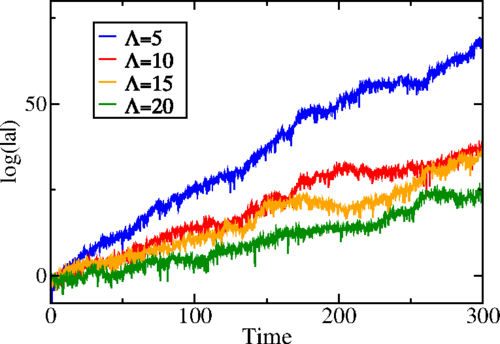
\includegraphics[width=\linewidth]{./graphics/FIG.4.png}
\end{column}
\begin{column}{.49\textwidth}
Fitting $\rfun{\ln}{\hH/\varLambda}$ gives $\alpha$ and $\beta$\\
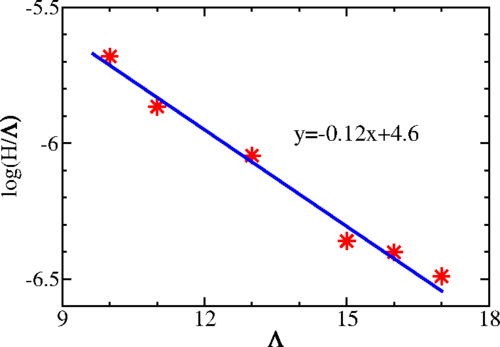
\includegraphics[width=\linewidth]{./graphics/FIG.6.png}
\end{column}

\end{columns}

\end{frame}



\section{Summary and comments}

\begin{frame}{Summary}

  % Keep the summary *very short*.
\begin{itemize}
\item Making of the oscillator equation \cref{eq:sho}:
\begin{enumerate}
\item Quantised Klein--Gordon field in flat space-time
\item Classical, localised Robertson--Walker metric
\end{enumerate}
\item Solving  the oscillator equation \cref{eq:sho}:
\begin{enumerate}
\item Ignoring the Stochasticity in most calculation
\item Parametric oscillation
\item WKB approximation
\item Adiabatic approximation
\end{enumerate}
\item Validation of the various approximation: numerics

\item Summarised up to eq.~(75); The rest (up to eq.~(214); 3 appendixes) 
contains more details and discussions
\end{itemize}
  
  % The following outlook is optional.
  %\vskip0pt plus.5fill
\end{frame}

\begin{frame}{Comments}

  % Keep the summary *very short*.
\begin{itemize}
\item Differential equation with fluctuating coefficients: stochastic 
differential equation \cite{van-Kampen-2007}
\begin{itemize}
\item Famous case: Langevin equation for Brownian motion
\begin{equation}
m\dot {\vec v} + \lambda \vec v = \rfun{\vec \eta}{t}
\end{equation}

\end{itemize}
\item Harmonic oscillator with stochastic frequency: studied, e.g.\ 
\cite{Bourret_1973,Van_Kampen_1976}
\item Applying quantum fluctuation to semi-classical Einstein equation: 
studied, e.g.\ \cite{Hu_2008}

\end{itemize}
  
  % The following outlook is optional.
  %\vskip0pt plus.5fill
\end{frame}



% All of the following is optional and typically not needed. 
\appendix
\section<presentation>*{\appendixname}
\subsection<presentation>*{For Further Reading}

\begin{frame}[allowframebreaks]
  \frametitle<presentation>{For Further Reading}
    
%  \begin{thebibliography}{10}
    
  \beamertemplatebookbibitems
  % Start with overview books.
\printbibliography[type=book]

%  \bibitem{Author1990}
%    A.~Author.
%    \newblock {\em Handbook of Everything}.
%    \newblock Some Press, 1990.
 
    
  \beamertemplatearticlebibitems
  % Followed by interesting articles. Keep the list short. 
\printbibliography[nottype=book]

%  \bibitem{Someone2000}
%    S.~Someone.
%    \newblock On this and that.
%    \newblock {\em Journal of This and That}, 2(1):50--100,
%    2000.
%  \end{thebibliography}
\end{frame}

%\section<presentation>*{More on Trace Distance and Fidelity}






\end{document}


